\chapter{Project description}
\textit{This chapter seeks to explain the design and implementation of the project along with the tests used for improving the system.}
\section{Architecture}
The architecture of the system explains the principle design blocks and interfaces. The system consist of the CDU and a number of sensor nodes as seen on figure \ref{fig:systembdd}. The CDU is responsible for contacting the sensor nodes in order to collect and store the data that has been acquired by the sensor nodes. The sensor nodes sole responsibility is to acquire data.\\
The supply for the sensors nodes is taken from the custom power line communication bus. Communication signals between the CDU and sensor nodes are found on the bus as well.\\ 
\begin{figure}[H]
	\centering
	\includegraphics[width=.9\textwidth]{billeder/11ProjectDescription/systembdd}
	\caption{System overview}
	\label{fig:systembdd}
\end{figure}
The general interface in the system is the bus. The sensor nodes are chain connected to the bus. The B+ connected is connected to the S+ of the first sensor in the chain. The next sensor in the chain is then connected with S+ to the S- of the first sensor. The last sensor in the chain is connected with S- to the B- on the CDU.\\

\fixme{Skal det her være her?}
The CDU and the sensor nodes can be described as several layers with regards to communication as seen on figure \ref{fig:systemlayers}.
\begin{figure}[H]
	\centering
	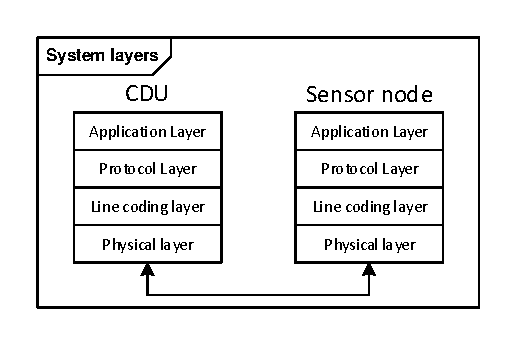
\includegraphics[width=.6\textwidth]{billeder/11ProjectDescription/System_Layers}
	\caption{System Layers}
	\label{fig:systemlayers}
\end{figure}

Principle designs of the different parts of the system are made by taking the blocks from the block definition diagram (figure \ref{fig:systembdd}) and creating internal block diagrams.\\
The CDU is comprised of six conceptual blocks as seen on figure \ref{CDU_IBD}. Each block has a unique responsibility. For instance the sensor power supply has the responsibility of powering the sensors. The sensor power supply and sensor communication makes up the physical layer with regards to figure \ref{fig:systemlayers}.

\begin{figure}[hbpt]
\centering
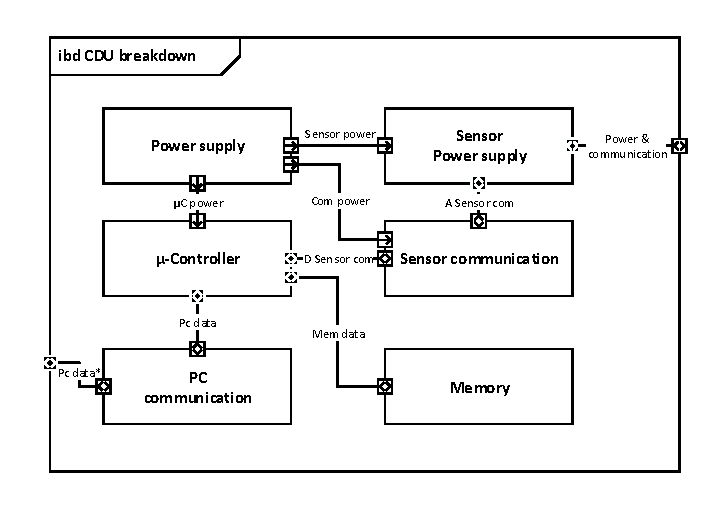
\includegraphics[width=.8\textwidth]{billeder/11ProjectDescription/CDU_IBD}
\caption{Internal Block Diagram of the CDU}
\label{CDU_IBD}
\end{figure}

\textbf{Noget om sensor note architecture.}\\




\begin{table}[H]
\centering
\begin{tabular}{|l|l|l|l|l|l|}
	\hline
	Start Sequence & Address & Function Code & DLM & Data & CRC  \\ \hline
	1 nibble & 1 nibble	& 1 nibble & 1 nibble & n bytes & 1 byte\\
	\hline
\end{tabular}
\caption{Message format for writing and reading}
\label{table:stdmsgtosensor}
\end{table}


\section{Design and implementation}
The design and implementation of the system is a naturally continuation of the technology study made in this project. The key part was integrating the acquired knowledge from the study and applying it to design and implement the prototype system.\\
When taking the system layers into consideration (figure \ref{fig:systemlayers}), the protocol and line coding layers fits well into software design. The physical layer matches hardware design and implementation.\\
The design of the physical hardware layer was derived from the technology study of how a communication bus could be made. The central parts of the communication is carrying the communication and the conversion from digital levels to something that can be carried by the bus.\\ 
The technology study led to a current loop being used to communicate with the sensor nodes. Two different current levels corresponds to logic 0(low) and 1(high). When responding, the sensor nodes use two different voltage levels.\\
The conversion from digital levels to analog current levels is handled by two block in the CDU: The Sensor power supply block (figure \ref{fig:CDUSPS}) and the Sensor communication block (figure \ref{fig:CDUSC}).\\
\begin{figure}[H]
	\begin{minipage}[b]{0.45\linewidth}
	\centering
	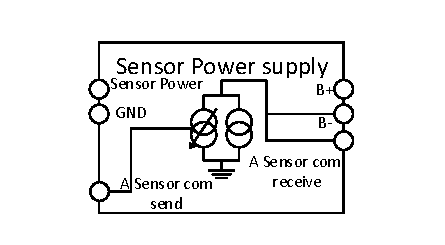
\includegraphics[scale=1]{billeder/11ProjectDescription/CDUSPS}
	\caption{Detailed CDU Sensor Power supply design.}
	\label{fig:CDUSPS}
	\end{minipage}
	\hspace{0.5cm}
	\begin{minipage}[b]{0.45\linewidth}
	\centering
	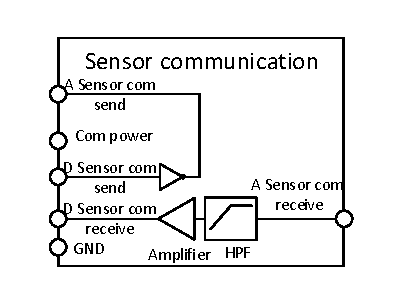
\includegraphics[scale=1]{billeder/11ProjectDescription/CDUSC}
	\caption{Detailed CDU Sensor communication design.}
	\label{fig:CDUSC}
	\end{minipage}
\end{figure}
Each sensor node will react to the difference in current levels. The current is converted to a voltage in the power supply block of the sensor node (figure \ref{fig:SN_PS_FIGURE}). The voltage levels are then converted to digital levels by the communication block of the sensor node(figure \ref{fig:SN_com_fig}). The digital levels are handled by the logic handler which will be described later in this chapter.\\
\begin{figure}[H]
	\begin{minipage}[b]{0.45\linewidth}
	\centering
	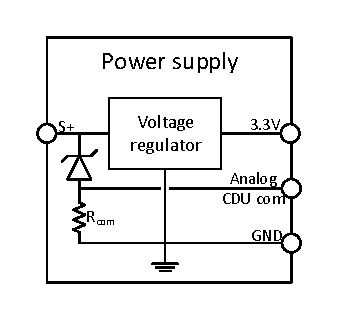
\includegraphics[width=0.8\textwidth]{billeder/11ProjectDescription/powersupply_detailed_sn}
	\caption{Sensor node power supply block}
	\label{fig:SN_PS_FIGURE}
	\end{minipage}
	\begin{minipage}[b]{0.45\linewidth}
	\centering
	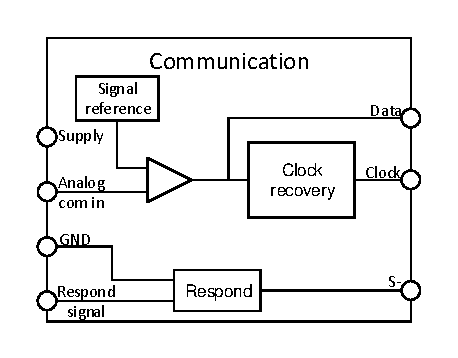
\includegraphics[width=1\textwidth]{billeder/11ProjectDescription/communication_sn}
	\caption{Sensor node communication block}
	\label{fig:SN_com_fig}
	\end{minipage}
\end{figure} 
Responding starts once the addressed sensor node has finished chewing through the message it has received. The digital level signal is converted to two different voltage levels by the communication block of the sensor node. The voltage levels on the bus is then directed from the sensor power supply of the CDU to the sensor communication block of CDU. The voltage levels will then be converted to digital logic levels and handled by the CDU.

\section{Tests}
